\documentclass[10pt,a4paper]{article}
\usepackage[english,swedish]{babel}
\usepackage{amsmath}
\usepackage{graphicx}
\usepackage{lmodern}
\usepackage[font=small,format=plain,labelfont=bf,up,textfont=it,up]{caption}
\usepackage[nottoc]{tocbibind}
\usepackage{url}
\usepackage{courier}
\usepackage[T1]{fontenc}
\usepackage[titles]{tocloft}
\usepackage{subfig}

\setcounter{secnumdepth}{5}
\setlength{\parindent}{0in}

\renewcommand{\topfraction}{0.85}
\renewcommand{\textfraction}{0.1}
\renewcommand{\floatpagefraction}{0.75}

\makeatletter
\newcommand\ackname{Acknowledgements}
\if@titlepage
  \newenvironment{acknowledgements}{
      \titlepage
      \null\vfil
      \@beginparpenalty\@lowpenalty
      \begin{center}%
        \bfseries \ackname
        \@endparpenalty\@M
      \end{center}}%
     {\par\vfil\null\endtitlepage}
\else
  \newenvironment{acknowledgements}{
      \if@twocolumn
        \section*{\abstractname}
      \else
        \small
        \begin{center}
          {\bfseries \ackname\vspace{-.5em}\vspace{\z@}}
        \end{center}
        \quotation
      \fi}
      {\if@twocolumn\else\endquotation\fi}
\fi
\makeatother

\title{CuEira, gene-enviroment interaction analysis on GPU}
\author{Daniel Berglund}
\date{March 2014}

\begin{document}
\maketitle

\clearpage
\selectlanguage{english}
\begin{abstract}
Abstract på svenska
\end{abstract}
\clearpage
\selectlanguage{english}
\begin{abstract}
Abstract in english
\end{abstract}
\clearpage
%\begin{acknowledgements}
%Asdf
%\end{acknowledgements}
%\clearpage
\tableofcontents
\newpage

\section{Introduction}
\subsection{Epidemiology}
Epidemiology combines several discplines, bioinformatics, computer science, statistics and sociology.

\cite{rothman1998modern,rothman2002intro_epidemiology}

\subsection{Genome-wide association studies}
Genome-wide association studies(GWAS) is a common type of study to search for associations between genetic markers and diseases. Classicaly it doesn't consider interaction between the genetic markers nor enviromental factors. Gene-gene interaction has started to become more common\cite{cordell_detect_review}, however gene-enviroment is still uncommon\cite{gene_enviroment_2013}. Interaction between genes and enviromental factors are considered imporant for complex diseas such as cancer and autoimmune diseases. \cite{cordell_detect_review, gene_enviroment_2013, geira, ra_smoking}\\
\\
Gene-gene interaction is constrained mostly by computational problems\cite{cordell_detect_review}. Gene-enviroment interaction faces a number of challegnes.



These types of studies are usually either cohort or case-control. In cohort studies a sample of a population who don't have the disease is followed. Variables that are suspected to be releveant for the disease is measured and over time some of the individuals will get the disease. The data collected can then be used to find risk factors. In case-control studies two groups are compared to find risk factors. One group consists of individuals with the disease and the other of individuals that are similar to the cases but that doesn't have the disease. \cite{rothman1998modern,mann_observational}\\
\\
The genetic markers are commonly single-nucleotide polymorphisms(SNPs). SNPs are variations in the genome where a single Nucleotide differs between individuals in a population\cite{fareed_snp}. Enviromental factors can be various things such as smoking, physical activity and so on. The amount of data is usually thousands individuals and hundred thousands or millions SNPs. Due to the high number of SNPs few programs investigate more than second order interaction, a few can handle more but not without drawbacks. \cite{gwis,high_order_2012,fast_high_order_cluster}.\\
\\
SNPs are binary variables which is an advantage that is often used when searching for gene-gene interaction. They are binary since the three possible combinations of allels(AA, Aa, aa)  can be represtend as 1,1,0 if its dominat model and 0,0,1 if its ressive\cite{}. Enviromental factors can be of any type\cite{gene_enviroment_2013}. Enviromental factors can also change over time(eg a person can stop smoking, move to a different area) while a persons genome reamains more or less constant.

\subsection{Defining Interaction}
What do we mean with interaction between factors? There are several definitions of the term\cite{rothman2002intro_epidemiology}. The overall goal is usually to find if \emph{biological} interaction is present. Biological interaction is when the factors co-operate through a physiological or biological mechanism and causes the effect (eg. Disease). This is useful since it's the true interaction in some sense and we can use it to explain the mechanisms involved and possibly find cures for diseas. However it's not well defined, it's not something we can calculate directly from data.\cite{rothman1998modern,rothman2002intro_epidemiology}\\
\\
\emph{Statistic} interaction on the other hand is much more well defined. However it's scale dependant, ie. interactions can appear and disappear based on transformations of the data. It also depends on the model used(eg Logistic, Linear). The common way to define statistic interaction is as the presence of product terms between the factors in the statistical model, this is refred to as \emph{multiplicative} interaction. For instance for a linear model $f(x,y)=ax+by+cxy+d$ c is the product term that implies multiplicative interaction between variables x and y. Statistic interaction is often called just interaction which can make it a  bit confusig.\cite{geira,rothman1998modern}\\
\\
It can also be defined as the divergence from additeve effects

It's called biological interaction by Rothman\cite{} and can also be called \emph{additive} interaction\cite{geira}. Here we we will use the term \emph{causual} interaction.\\

%Something about sufficnt cause?

\subsection{Confounders and Covarietes}
Confounding is one of the central issues in the design of epidemiologic studies. It's when the effect of the exposure is mixed with the effect of another variable. So if we don't measure the second variable the first effect would be estimated as stronger than it really is. The second varialbe is then a \emph{confounder}. Several methods in epidemiology are about avoiding or adjusting for confounding. Sometimes these variables needs to be incorperated into the models \cite{rothman2002intro_epidemiology}

\begin{figure}[h]
    \centering
    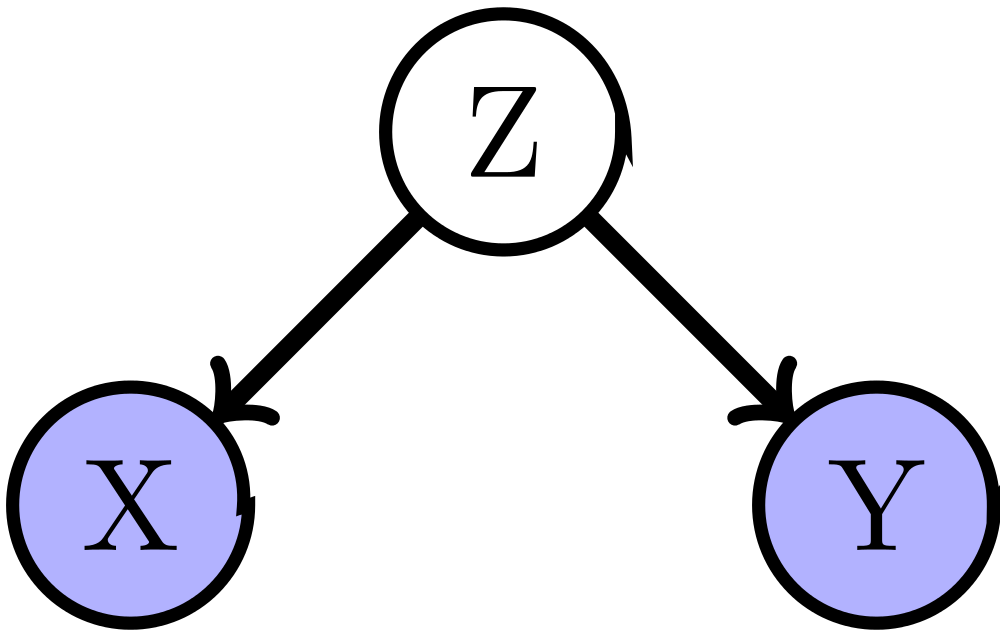
\includegraphics[width=5cm]{Simple_Confounding_Case.png}
    \caption{Illustration of a simple case of confounding. If we don't observe Z we might falesly find an association between X and Y. Picture from Wikipedia Commons.}
    \label{fig:awesome_image}
\end{figure}

 \cite{rothman1998modern}

Covarietes are similiar to confounders.

\subsection{GEIRA and JEIRA}
GEIRA is a tool for analysing gene-gene and gene-enviroment interaction. GEIRA uses additive interaction instead of multiplicative, commonly multiplicative interaction is used\cite{geira}. JEIRA is a parallelized immplementation of the enviromental interaction analysis in GEIRA. However it can only use one node.

\clearpage
\section{Background}
%Mathematical and physical bck (equations etc.)
%Algorithmic bck and concepts (e.g scalability, speedup etc.)
%computer architecture bck(describe CPU and GPU differences etc.)

There are a lot of algorithms and programs proposed for searching for interaction. They can be rougly classiefed into four categories, exhaustive, stochastic, machine learning/data mining and stepwise\cite{fast_high_order_cluster}. One of the big differences between methods is wether they are testing for interaction or testing for allowing interaction, see section \ref{test_type} for details. In short it's bla bla\\
\\
Exhaustive search is the most obvious approach, they compare all combinations of the SNPs in the data. They don't risk missing a combination but it also means they can be slow. Multifactor-Dimensionality Reduction(MDR)\cite{mdr_2001} and BOOST\cite{boost_gene_gene} are two examples.
\\
Stochastic methods uses random sampling to walk throught the data. BEAM\cite{beam_2007} is one example and it uses Markov Chain Monte Carlo(MCMC) to .
\\
Machine Learning and Data Mining methods are 
MDR\cite{mdr_2001} and Random Forest\cite{random_jungle}
\\
Stepwise approaches uses a filtering stage and a search stage. At the filtering stage uninterestings combinations are filtered out by using some exhaustive method. The other SNPs are the examined more carefully in the search stage. BOOST\cite{boost_gene_gene} is an example.
\\
Most research have focused on gene-gene interaction so there are few tools for gene-enviroment. Gene-gene interaction tools can sometimes be used to find gene-enviroment interaction, however they usually require the variable to be binary or have other problems since they weren't designed for gene-enviroment interaction\cite{gene_enviroment_2013}.\\
\\
Both CPU clusters\cite{biforce} and GPUs\cite{gwis,gboost,gmdr_gpu,cuda_lr,genie_2012} have been used for GWAS but GPUs are the most popular choice. Most of the methods for searching for interaction are inherintly good on GPUs because each combination can usually be considered independtly from the others. More about this in the section about computer architecture.

\subsection{Contingency Tables}
A contingency table is a matrix used to describe categorical data. Each cell contains the frequency of occurances with a specific combination of variables. Table \ref{table:contingency_table} is an example of an 2 x 3 table. From it we can for instance see that 171 persons that got the placebo had an nonfatal attack. Contingency tables are the basis for various statistical tests to model the data. Contingency tables can be used directly for tests like $chi^2$. \cite{agresti_categorical}

\begin{table}[h]
\begin{tabular}{ l c c c }
  \hline
  & Fatal Attack & Nonfatal Attack & No Attack\\
  \hline
  Placebo & 18 & 171 & 10 845 \\
  Aspirin & 5 & 99 & 10 933 \\
  \hline  
\end{tabular}
\caption{Contingency table describing the outcome of a medical study, from \cite{agresti_categorical}}
\label{table:contingency_table}
\end{table}

\subsubsection{Logisitic and Log-linear Regression}
For logisic regression its Binomial\cite{agresti_categorical}

log lineare is Possion\cite{agresti_categorical}

\subsubsection{Weighted Logistic Regression}
Need to find the details on this.

\subsubsection{Statistic Measures}
Relative risk and odds ratio\cite{agresti_categorical}

relative risk due to interaction

AP

Causual bond things

\subsection{Data Mining Approaches}
Approaches based on Data Mining and Machine Learning have been a popular choice for GWAS. Multifactor-Dimensionality Reduction(MDR)\cite{mdr_2001} and Random Forest(RF)\cite{random_forest} are among the most common\cite{gene_enviroment_2013,cordell_detect_review}. There are others as well such as clustering approaches \cite{fast_high_order_cluster}. Most of the are used for screening the data for possible interactions\cite{gene_enviroment_2013,cordell_detect_review}.\\
\\
Their biggest advantage is that they are usually nonparametric, model free and designed with high dimensional data in mind.
\\
However they are prone to overfitting and the usual way to try to prevent that is to use cross valdiation and sometimes permutation tests. That means that even if the method itself is fast it's repeated so many times that it can be slow in the end\cite{cordell_detect_review}.

\subsubsection{Multifactor-Dimensionality Reduction}
Multifactor-Dimensionality Reduction(MDR) is \cite{mdr_2001}
It has been used for gene-enviroment interaction\cite{gene_enviroment_2013}

\subsubsection{Random Forest}
Random Forest(RF) is an ensemble learning method, ensemble metods combine multiple models to improve performance. It takes bootstrap samples of the data and builds descion trees on them. The trees are then combined to from the classifier. Usually hundres or thousands of trees are used depending on the problem\cite{random_forest}. One of the most popular variants of Random Forest for GWAS is Random Jungle.\cite{random_jungle}
\\
It has been shown in high dimensional data that it tends to only rank interacting factors high if they have strong marginal effects\cite{winham_rf_2012}. Also the ranking of the variables doesn't say which factor it's interacting with either since it's based on the joint distributions\cite{gene_enviroment_2013}. How to incorperate the enviromental factors in RF is also not trivial, using variables with very different scales can bias the results\cite{gene_enviroment_2013}.

%\subsection{Cross Validation, Boosting and Permutation Tests}
%Cross Validation is a common technique for validation in Machine Learning.\\
%\\
%Boosting and Permutation Tests are similar to each other.

\subsection{Test for interaction vs Test for allowing interaction}
\label{test_type}
Test for interaction is the test for the interaction parameter equal zero or not. Aka test saturated vs homogenous assocation\cite{boost_gene_gene}.

Test for allowing interaction on the other hand is . Aka test saturated vs block independance\cite{boost_gene_gene}.

This means that test for allowing for interaction is easeier and faster to use so it's commonly used for screening methods. 

hur funkar det med machine learning approaches?

\clearpage
\subsection{Computer Architecture}

\subsubsection{CPU}
branch prediction
prefetching

\subsubsection{GPU}
how do they look/work?

cuda\cite{cuda}

\paragraph{CUDA libraries}
-cublas
-magma
-thrust
-parray
-culatools

\paragraph{Effcient CUDA}
One of the main critizm against GPUs for general computing purposes is that it's hard to get good performance because it requires good knowledge about details of the GPU architecture, especially the memory architecture. There are a few things to keep in minde when writing CUDA programs.\\
\\
assync memory
-streams, conccurent kernels

avoid bank conflicts

little communctiation

minmize divergence

use correct memory
-global
-shared
-constant

textures
-previously imporant, doesn't matter much on modern gpus

other
-message parrsing, openMPI
-lib verbs, infiband
-pthreads
-openMP

\cite{cuda, cuda_best_practice}

\subsection{Performance Measures}
law thingy

speedup

scalability

\subsubsection{Clusters}
Shared memory

Message parsing

Low level, infiband verbs

Mix of gpus and cpu, top 500

\subsection{Which program for GPU and which for CPU?}
NVIDIA vs Intel performance claims, intel gets much lower than Nvidia. But who can you trust really?

Xeon Phi

GPUs loses more when going from single precision to double than CPUs. Peak performance on tesla-kepler cards for single precision is around 4 Tflops while double precision is around 1.4 Tflops. \cite{nvtesla}\\ cite the table thing

\section{Algorithm}
%Algorithm (up till 20 pages)
%  - Current state - Basic algorithm, Data structure, memory consumption, parallelization, load balancing and scalability
%  - And the same for own your implementation

%CURRENT

\subsection{Why GPU for GWAS?}
Most approaches to interaction analysis is embarasingly parallel since they considere each combination independtly from the others. 

Lots and lots of combinations. GPUs provided a lot of power compared to CPU. They are proven for GWAS. Lots of use with high gains.

\subsection{Current algorithm}
%problem with exathsutive

%memory problems(GENIE, CUDALR and so on)

%2 bit 3 bit data storage

%two stage analysis

%\subsection{Mine}
%exhaustive and second stage.

%first stage if there is time.

\section{Results}
%Results (up till 15 pages including plots)
%  - Performance measurements (scalability, speedup and efficiency as well as load balancing)
%  - Setup(simulation setup, compilers and hardware setup)
%  - Single node performance
%  - multy-node performance


\section{Discussion and Conclusions}
%Discussion and Conclusions (up to 3 pages)


\section{Outlook}
%Outlook (up to one page)

\section{Appendix}
%List of figs
%List of tables


\newpage
\bibliographystyle{ieeetr}
\bibliography{hpc.bib,statistics.bib,misc.bib}
\end{document}